%===============================================================
% Author: Rodolfo Ferro Pérez
% Email: ferro@cimat.mx
% Twitter: @FerroRodolfo
%
% ABOUT COPYING OR USING PARTIAL INFORMATION:
% This document was originally created by Rodolfo Ferro, for
% his talk in FLISoL 2017 at Instituto Tecnológico de León.
% Any usage of this document or its contents must be granted by
% the author. You can contact him via email or Twitter.
%===============================================================

\documentclass[usenames,dvipsnames]{beamer}
\usetheme{metropolis} % Use metropolis theme

% Import packages:
\usepackage[many]{tcolorbox}
\usepackage{wrapfig}

\title{Primeros pasos con Python:}
\subtitle{Manipulando imágenes}
\author{Rodolfo Ferro\\{\footnotesize \textcolor{Turquoise}{\textsc{@FerroRodolfo}}}}
\institute{Universidad de Guanajuato\\ CIMAT A.C.\\
\begin{wrapfigure}{r}{0.3\textwidth}
  \vspace{-30pt}
  \begin{center}
    % \hspace*{-2cm}
    
\includegraphics[width=0.3\textwidth]{imgs/flisol}
    % \hspace*{-6.3cm}
    % 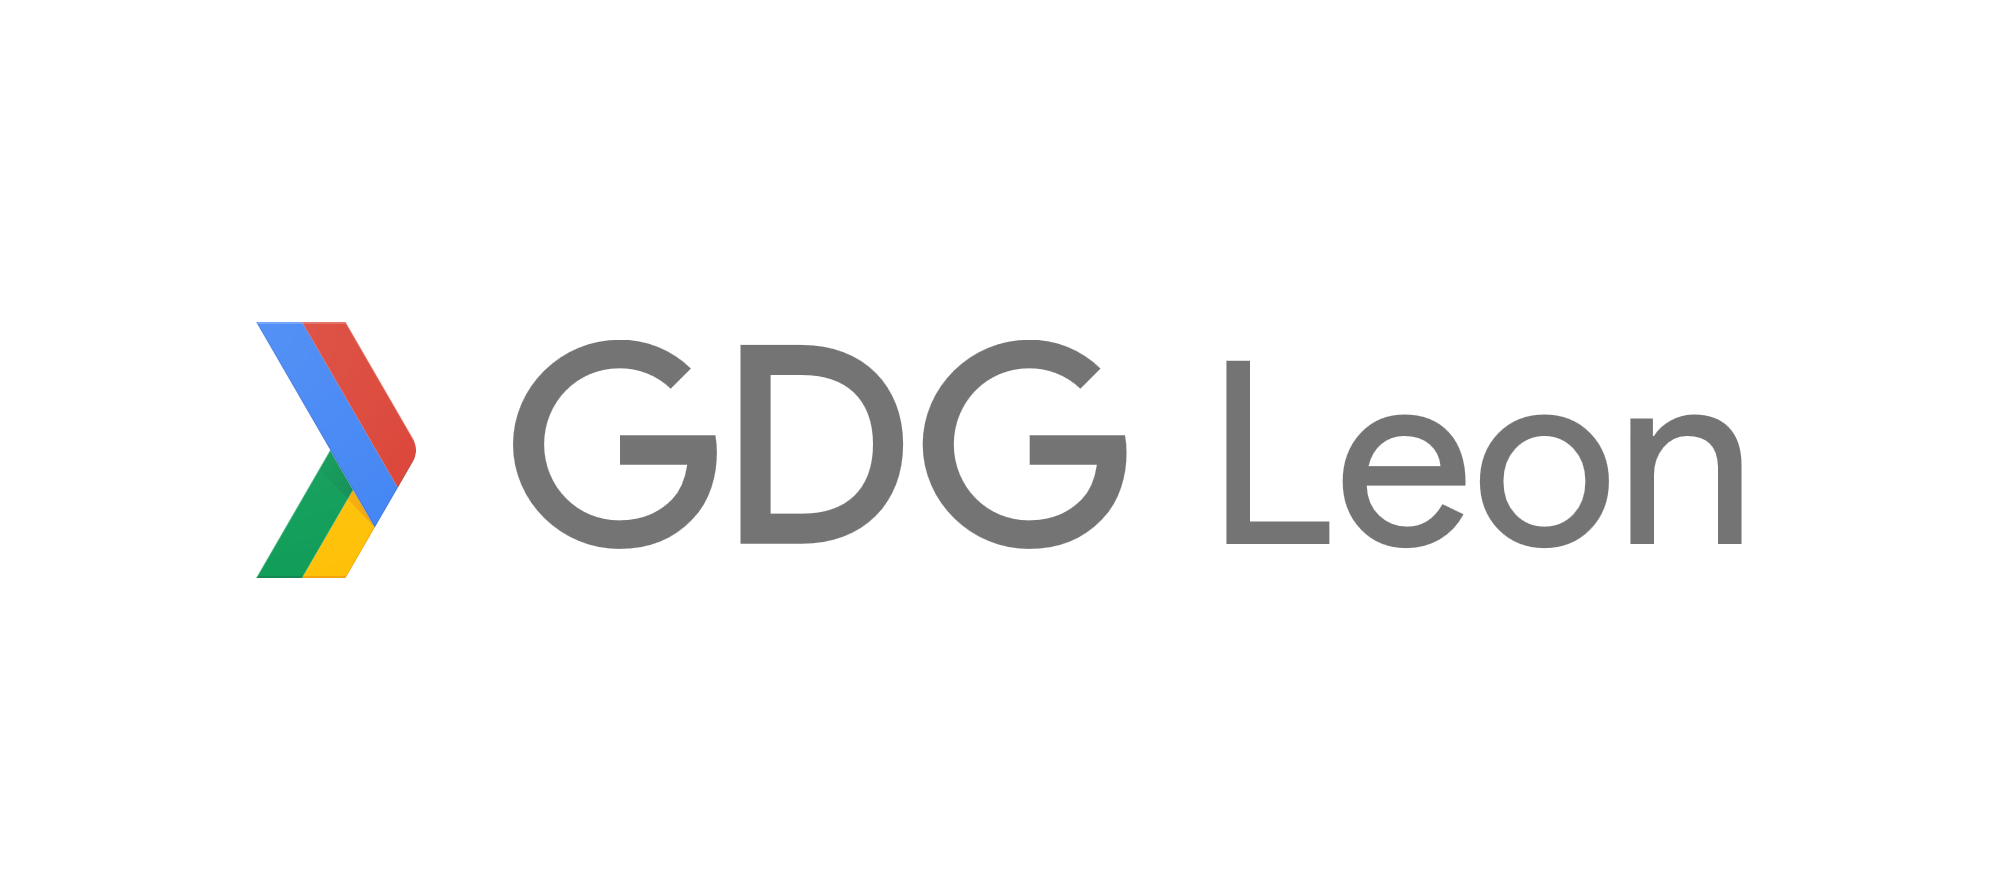
\includegraphics[width=0.3\textwidth]{imgs/GDGLeon}
  \end{center}
\end{wrapfigure}
}
\date{Abril 29, 2017}
\begin{document}
  % Title slide:
  \maketitle

  % Table of contents:
  \begin{frame}{Tabla de contenido}
    \setbeamertemplate{section in toc}[sections numbered]
    \tableofcontents[hideallsubsections]
  \end{frame}

  % First section: Acerca de Python
  \section{Sobre Python}
  \begin{frame}[standout]
    \textit{Python es un lenguaje interpretado, sencillo, versátil y poderoso.
    La belleza del lenguaje radica en su sintaxis.}\\
    \vspace{1.4cm}
    
\includegraphics[scale=0.02]{imgs/python}
  \end{frame}

  \begin{frame}{Un poco de historia (I)}
    \begin{itemize}
      \item Python fue creado a inicios de los 90's por Guido van Rossum en el
      \textit{Stichting Mathematisch Centrum} (CWI), en los Países Bajos, como
      un sucesor del lenguaje ABC.

      \item Guido sigue siendo el principal autor, aunque incluye muchas
      contribuciones por parte de otros.
    \end{itemize}
  \end{frame}

  \begin{frame}{Un poco de historia (II)}
    \begin{itemize}
      \item En mayo del 2000, Guido y el equipo core de desarrollo de Python
      se mudan a \textit{BeOpen.com} para formar el equipo {BeOpen PythonLabs}.

      \item En octubre del mismo año, los PythonLabs se mudan a Digital Creations
      (hoy Zope Corporation) y en 2001 se crea la \textit{Python Software Foundation}
      (PSF), una organización sin fines de lucro creada específicamente para
      poseer todo lo relacionado con propiedad intelectial sobre Python.
    \end{itemize}
  \end{frame}

  \begin{frame}{Python en el mundo del SL}
    \begin{itemize}
      \item Todos los releases de Python son Open Source.
      \item De acuerdo a la \textit{Free Software Foundation}:
    \end{itemize}
    \begin{center}
      \begin{tcolorbox}[beamer,
                  width=1.065\textheight,
                  arc=0pt,
                  boxsep=0pt,
                  left=0pt,right=0pt,top=0pt,bottom=0pt,
                  ]
        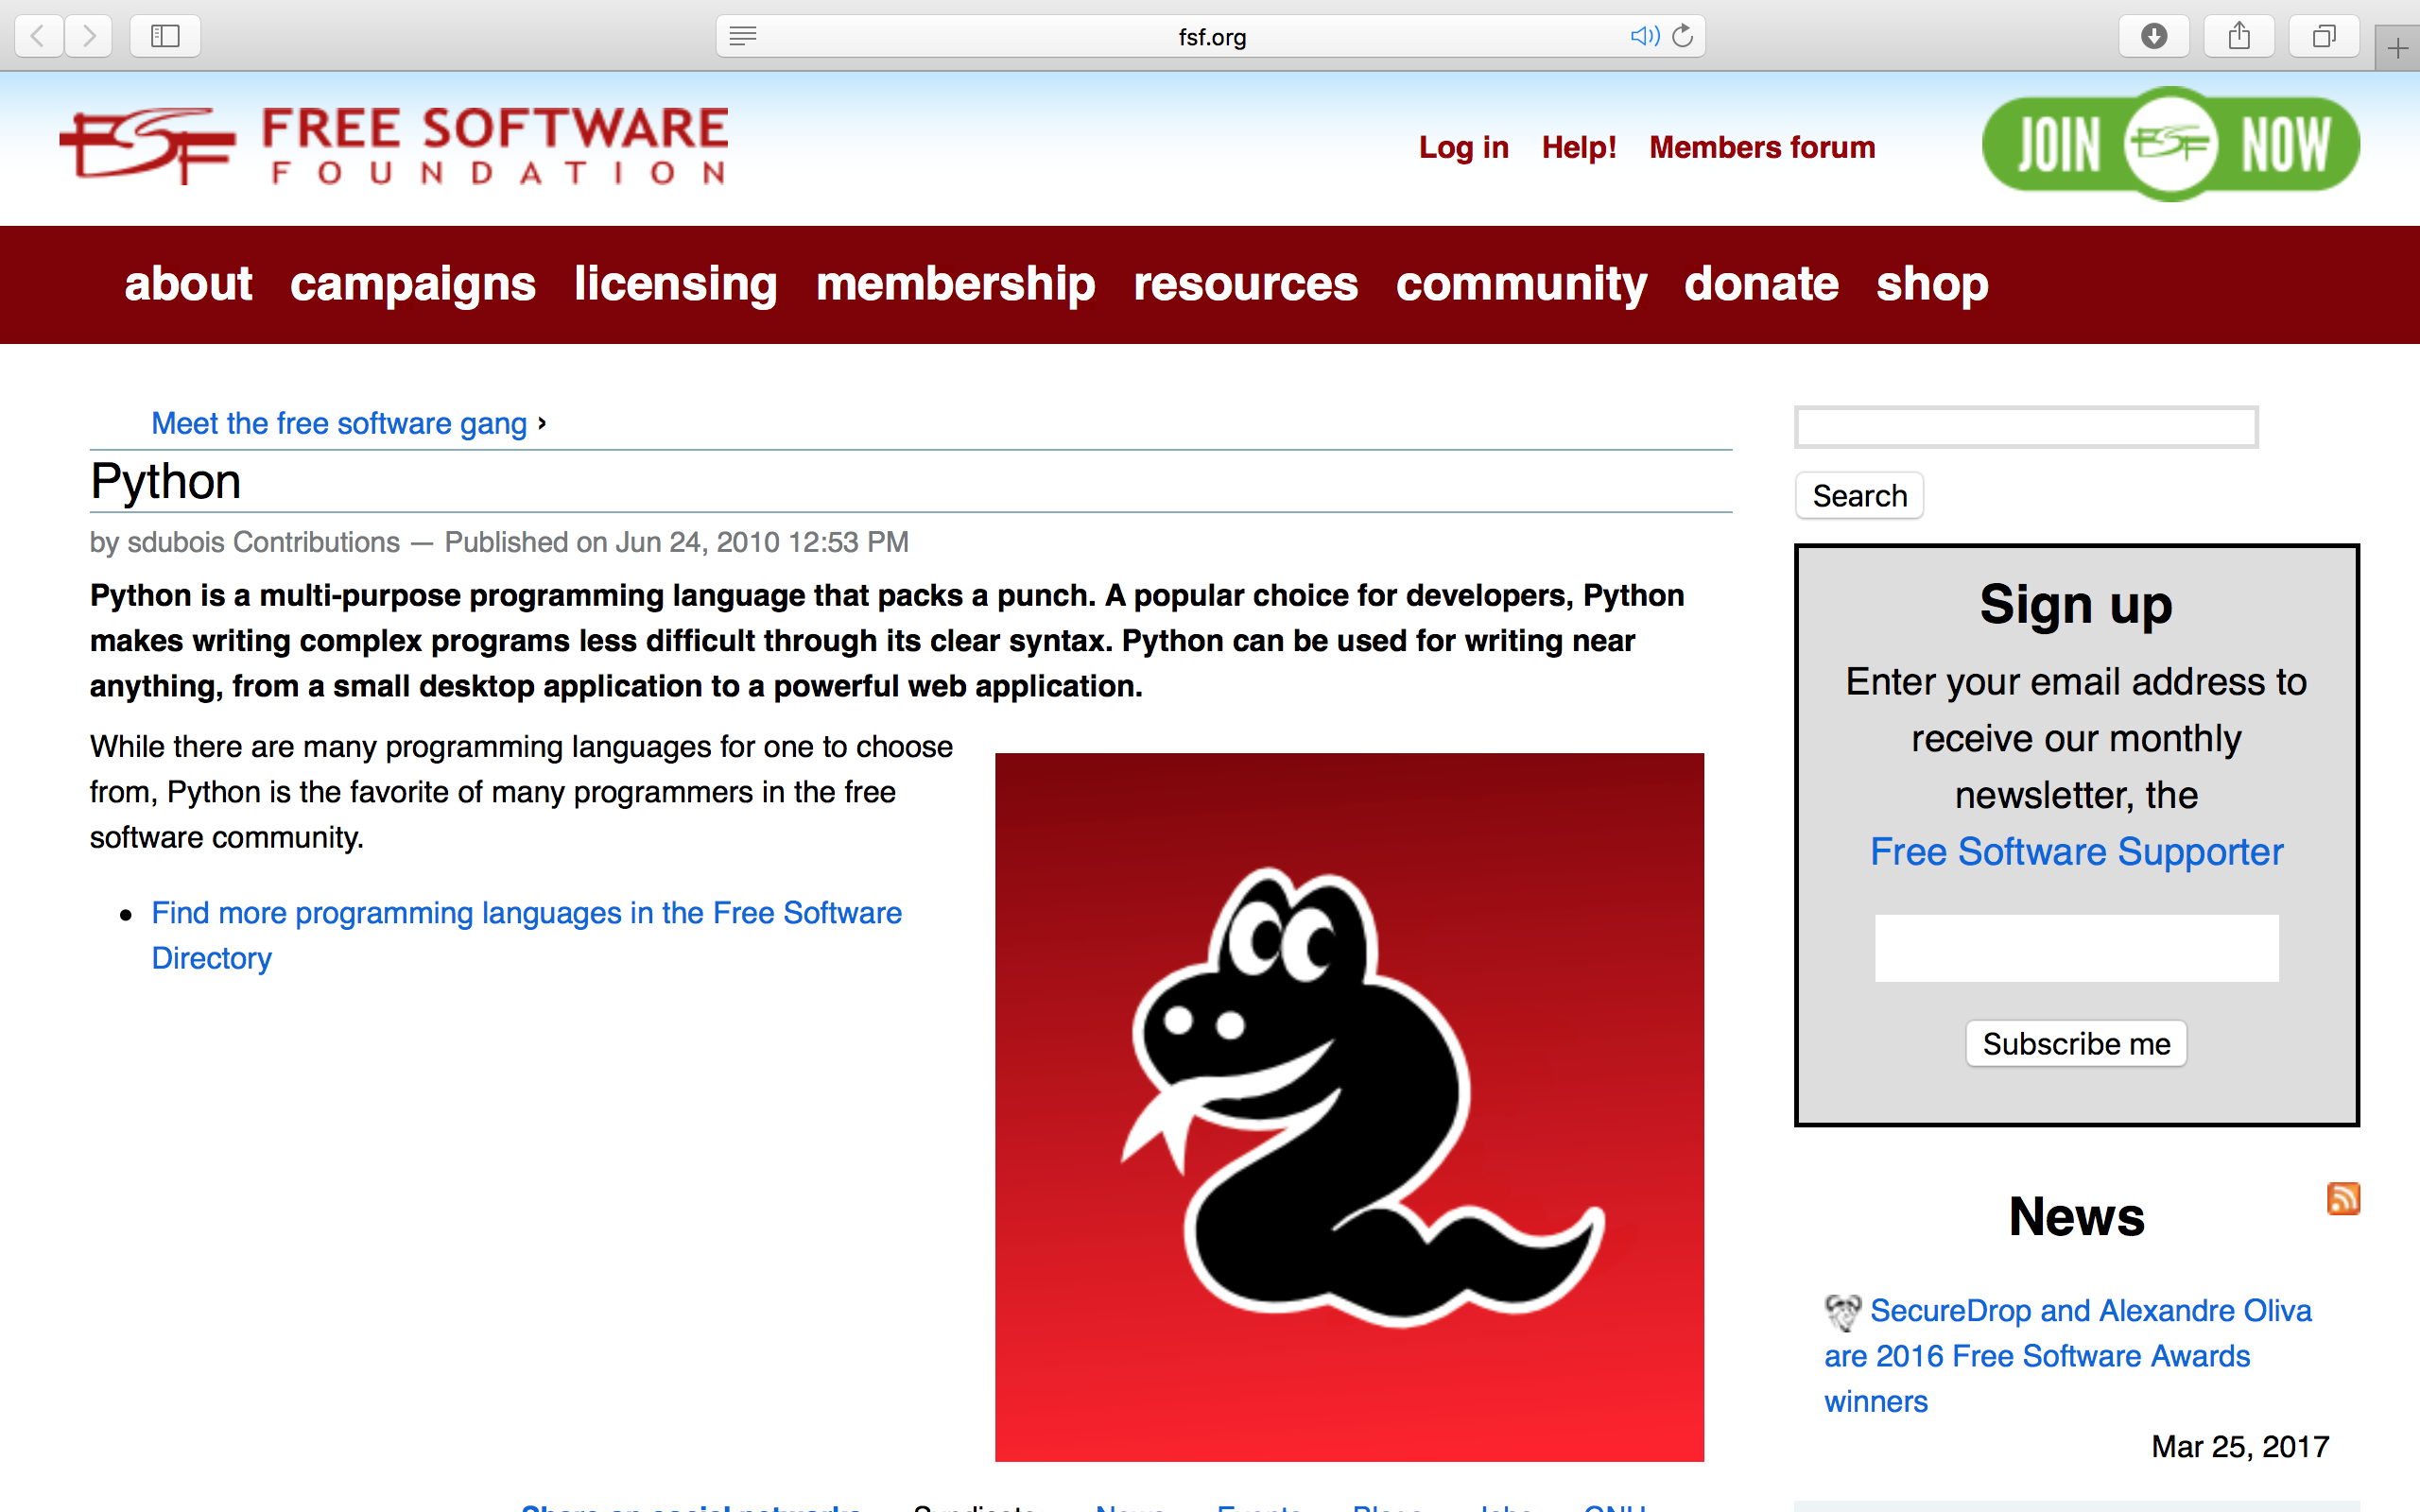
\includegraphics[scale=0.2]{imgs/fsf}
      \end{tcolorbox}
    \end{center}
  \end{frame}

  \begin{frame}{Recordando un poco...}
    Un \textbf{Software Libre} es aquel que respeta las cuatro libertades que
    la \textit{FSF} establece:
    \begin{itemize}
      \item La libertad de usar el programa con cualquier propósito.
      \item La libertad de estudiar cómo funciona el programa y modificarlo,
      adaptándolo a tus necesidades.
      \item La libertad de distribuir copias del programa, con lo cual puedes
      ayudar a tu prójimo.
      \item La libertad de mejorar el programa y hacer públicas esas mejoras a
      los demás, de modo que toda la comunidad se beneficie.
    \end{itemize}
    \textbf{Nota:} El Software Libre no es necesariamente gratuito.
  \end{frame}

  % Second section: Instalación
  \section{Instalación}
  \begin{frame}{Instalando Python}
    \begin{itemize}
      \item Ir al sitio oficial: {\color{RoyalBlue} \url{https://www.python.org/downloads/}}
      \item Descargar la versión 3.6.x.
    \end{itemize}
    \begin{center}
      \begin{tcolorbox}[beamer,
                  width=1.065\textheight,
                  arc=0pt,
                  boxsep=0pt,
                  left=0pt,right=0pt,top=0pt,bottom=0pt,
                  ]
        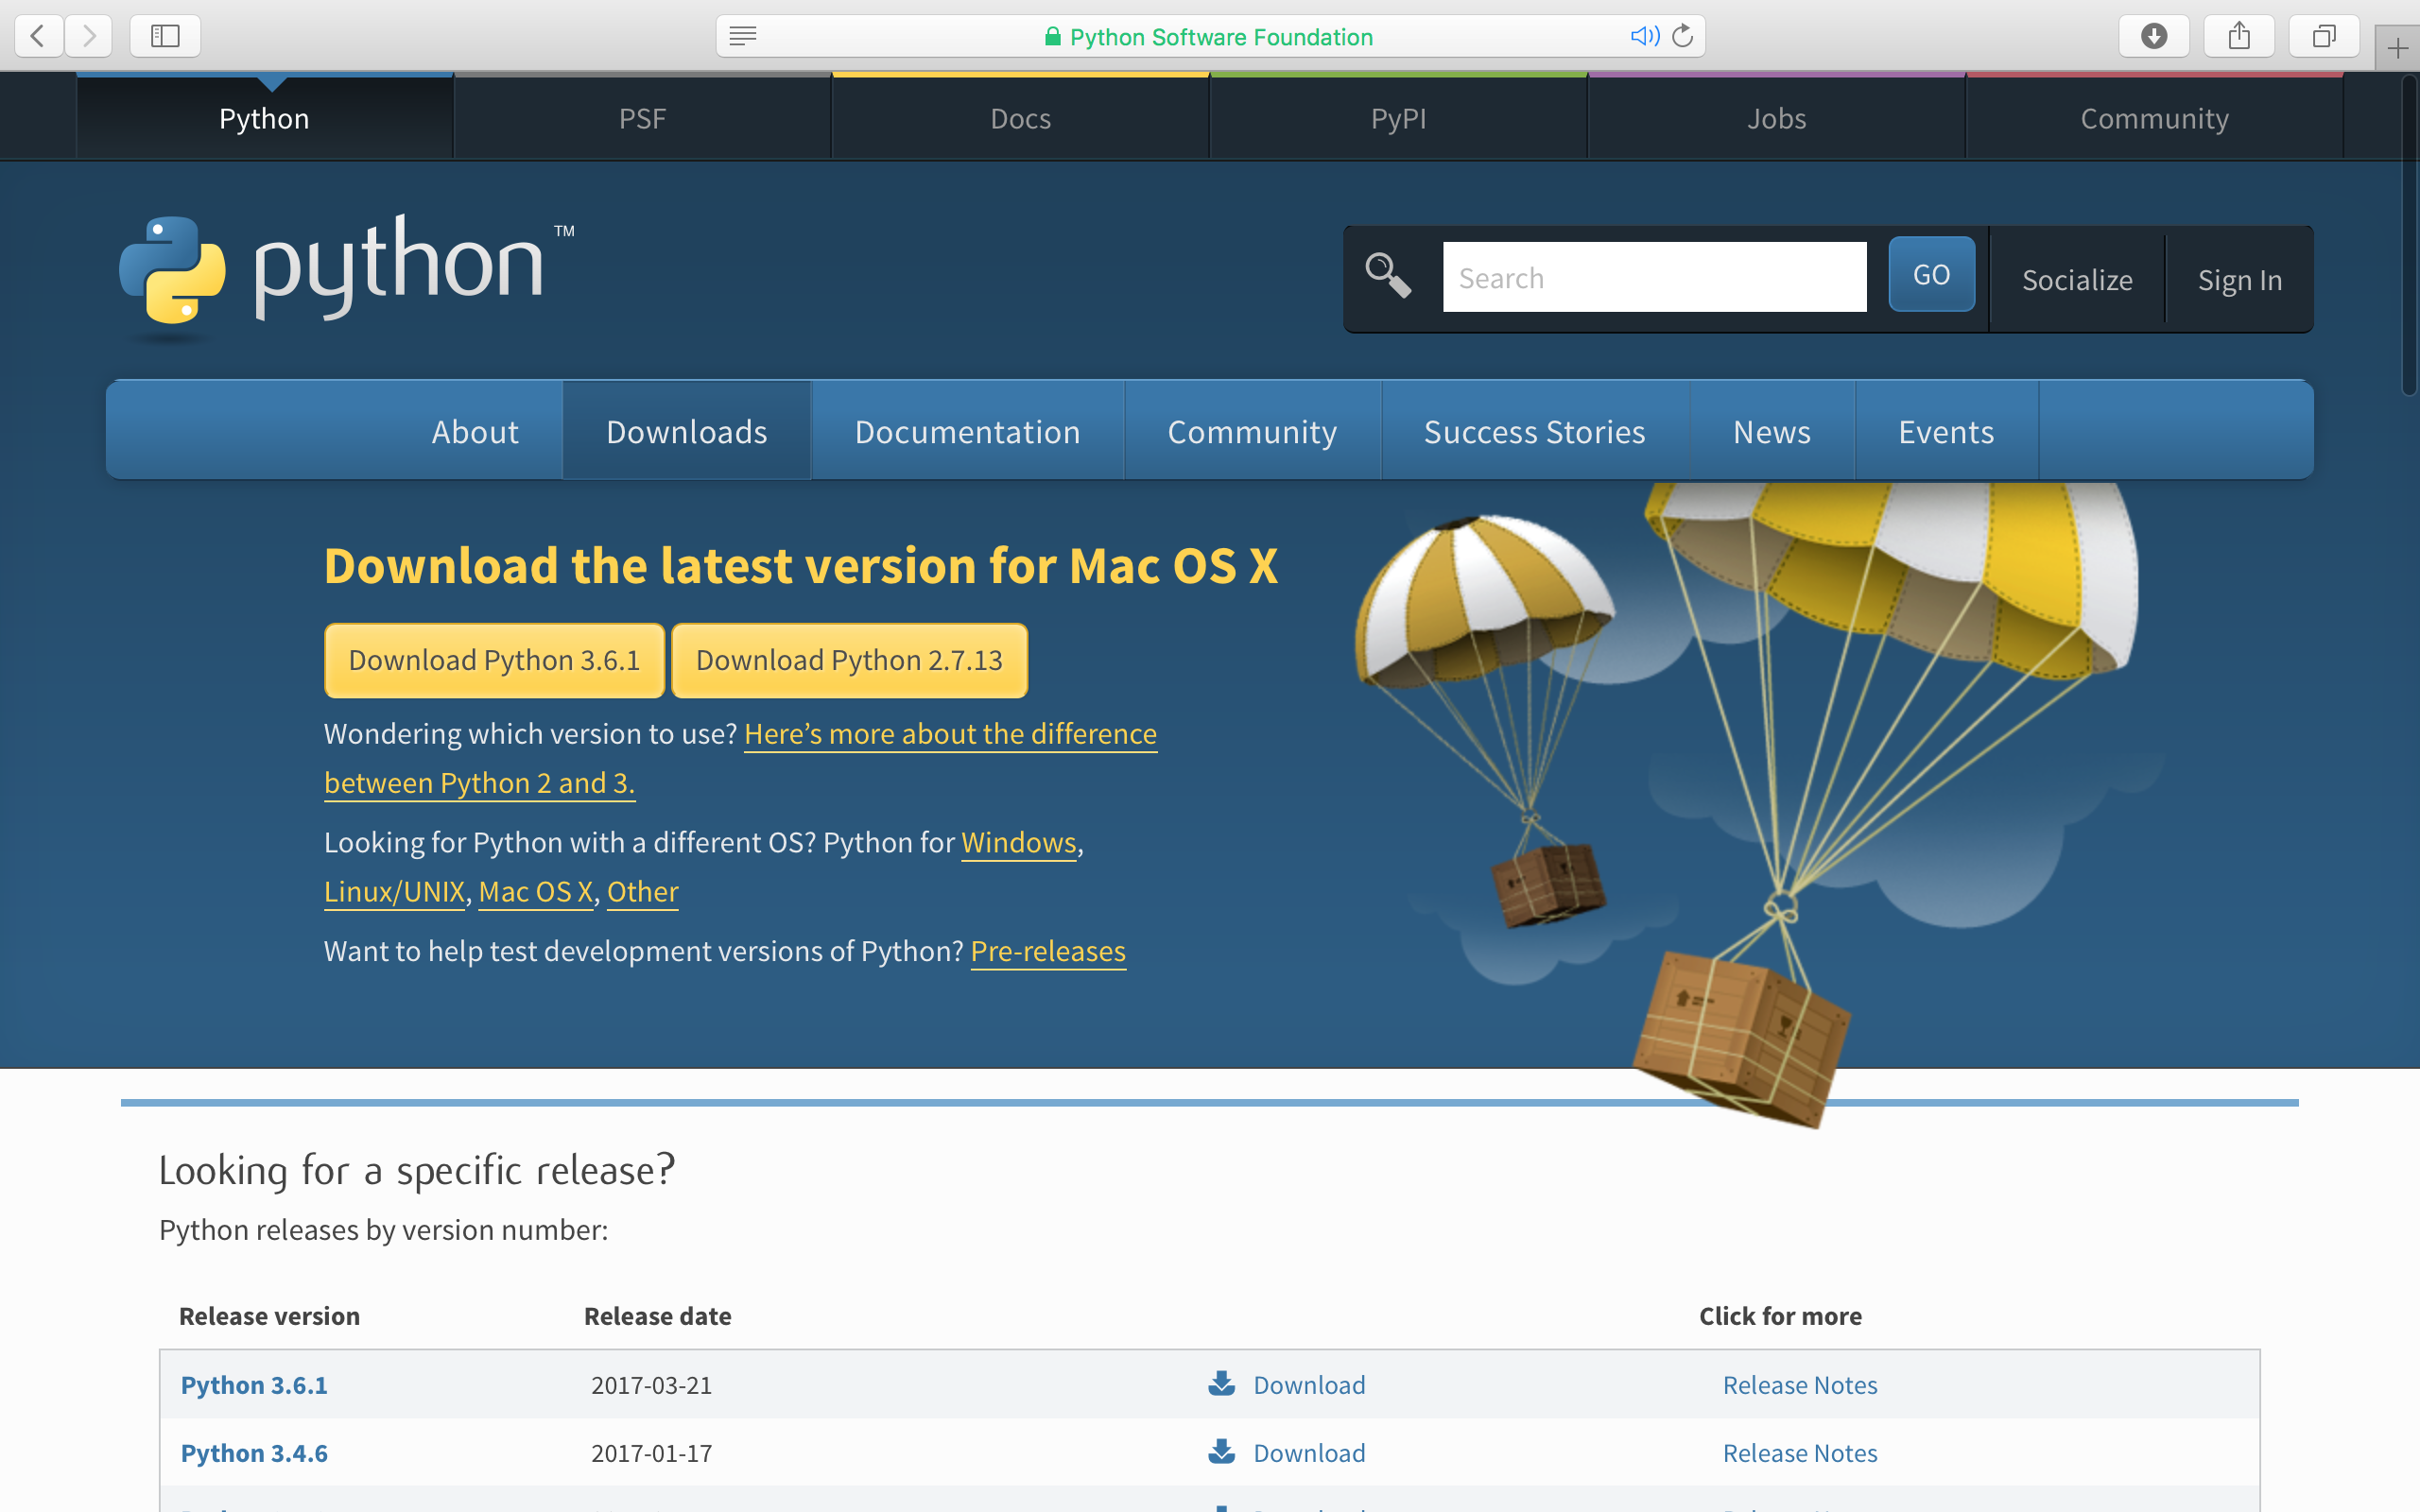
\includegraphics[scale=0.2]{imgs/download}
      \end{tcolorbox}
    \end{center}
  \end{frame}

  \begin{frame}{Instalando Python}
    \textbf{En Windows:}
    \begin{itemize}
      \item Preferentemente instalarlo en el disco local \texttt{C://}.
      \item Dar check a la opción "Add Python to PATH".
    \end{itemize}
    \textbf{En Linux/Unix:}
    \begin{itemize}
      \item No hace falta algo adicional, todo es hermoso.
      \item Es más, por default ya viene instalada la versión 2.7 de Python.
    \end{itemize}
  \end{frame}

  \begin{frame}{Instalando paquetes}
    Al instalar Python, se instala \texttt{pip} (\textit{Python Package Index}),
    que es un gestor de paquetes de Python. Usando \texttt{pip} instalaremos:
    \begin{itemize}
      \item \textbf{NumPy}, que incluye herramientas de métodos numéricos.
      \item \textbf{Matplotlib}, que incluye herramientas de visualización.
    \end{itemize}
    \textbf{Nota:} Python se instala con su librería estándar. Lo recomendable
    es instalar una distribución (como \textit{Anaconda}) para una mejor
    gestión de paquetes, además de instalarse por default los más usados.
  \end{frame}

  \begin{frame}{Paquetes de manipulación de imágenes}
    Existen diversos paquetes para manipular imágenes:
    \begin{itemize}
      \item \textbf{PIL} (\textit{Python Imaging Library})
      \item \textbf{OpenCV} (\textit{OpenSource Computer Vision})
      \item \textbf{scikit-image} (\textit{Scientific Kit - Image})
      \item Etc.
    \end{itemize}
    Cada uno trata de manera distinta las imágenes y se enfocan en cosas
    diferentes. Como es un taller de primeros pasos, no usaremos alguno de
    estos paquetes, sino que trabajaremos desde cero, sólo con \textbf{numpy}
    y \textbf{matplotlib}.
  \end{frame}

  \begin{frame}{Instalando \textbf{numpy} y \textbf{matplotlib}}
    Abriremos una consola y ejecutaremos los siguientes comandos.
    \metroset{block=fill}
    \begin{block}{Para instalar \textbf{numpy}:}
      \texttt{\$\hspace{0.3cm}sudo pip install numpy}
    \end{block}
    \vspace*{0.5cm}
    \begin{block}{Para instalar \textbf{matplotlib}:}
      \texttt{\$\hspace{0.3cm}sudo pip install matplotlib}
    \end{block}
    \textbf{Nota:} En Windows se omite el comando \texttt{sudo}.
  \end{frame}

  % Third section: Primeros pasos
  \section{Primeros pasos}
  \begin{frame}{Lo básico (I)}
    La belleza de Python radica en la sintaxis, los bloques de código deben
    tener la misma indentación, pues las llaves \{ \} se utilizan para una
    estructura de datos (diccionarios).\\

    \vspace*{0.5cm}
    \metroset{block=fill}
    \begin{block}{Un ejemplo:}
        \hspace{0.7cm}{\color{LimeGreen} \texttt{while }}{\color{Cerulean} \texttt{True}}{\color{LimeGreen} \texttt{:}}\\
        \hspace{1.4cm}{\color{lightgray} \texttt{\# El bloque de código dentro del ciclo debe}}\\
        \hspace{1.4cm}{\color{lightgray} \texttt{\# estar en el mismo nivel de indentación}}\\
        \vspace*{0.5cm}
        \hspace{1.4cm}{\color{LimeGreen} \texttt{print}}{\color{gray} \texttt{(}}{\color{ForestGreen} \texttt{"Infinite loop."}}{\color{gray} \texttt{)}}\\
        \vspace*{0.5cm}
    \end{block}
  \end{frame}

  \begin{frame}{Lo básico (II)}
    \begin{itemize}
      \item No hace falta terminar cada línea con punto y coma.
      \item Los scripts de Python pueden ejecutarse desde consola, usando un IDE o con
      Jupyter notebooks.
      \item Todos los scripts de Python deben ser de extensión .py (excepto por los
      Jupyter notebooks).
      \item Para fines prácticos, nosotros correremos scripts desde consola y
      escribiremos código desde un bloc de notas, por lo que es recomendable
      instalar uno tipo Atom o Sublime Text.
    \end{itemize}
  \end{frame}

  \begin{frame}{Variables y operaciones (I)}
    \begin{itemize}
      \item Las variables no se declaran, sólo se definen y Python sabe el
      tipo de variable que se está utilizando.
      \item Python cuenta con 5 tipos de datos estándar: números, cadenas
      de texto, listas, tuplas y diccionarios.
      \item Puedes realizar asignación múltiple.
      \item Las operaciones básicas con números son: +, -, *, /, //, **.
      \item En las cadenas de texto también puede usarse + (concatenación)
      y * (repetición).
    \end{itemize}
  \end{frame}

  \begin{frame}{Variables y operaciones (II)}
    Los tipos de variables que existen en Python son:
    \begin{itemize}
      \item \textbf{Enteros}, como 3.
      \item \textbf{Longs}, como 51924361L.
      \item \textbf{Flotantes}, como 3.14e4.
      \item \textbf{Complejos}, como 4.53-7j.
      \item \textbf{Strings}, como "Hola mundo".
      \item \textbf{Listas}, como [1., 3, 5.3, "perrito"].
      \item \textbf{Tuplas}, como (1., 3, 5.3, "perrito").
      \item \textbf{Diccionarios}, como \{"Nombre":"Rodolfo", "Apellido":"Ferro"\}
    \end{itemize}
  \end{frame}

  \begin{frame}{Condicionales}
    La sintaxis correspondiente es:
    \metroset{block=fill}
    \begin{block}{if/elif/else}
      \hspace{0.7cm}{\color{LimeGreen} \texttt{if }}{\color{Cerulean} \texttt{condition}}{\color{LimeGreen} \texttt{:}}\\
      \hspace{1.4cm}{\color{lightgray} \texttt{\# Block content}}\\
      \hspace{0.7cm}{\color{LimeGreen} \texttt{elif }}{\color{Cerulean} \texttt{condition}}{\color{LimeGreen} \texttt{:}}\\
      \hspace{1.4cm}{\color{lightgray} \texttt{\# Block content}}\\
      \hspace{0.7cm}{\color{LimeGreen} \texttt{else: }}\\
      \hspace{1.4cm}{\color{lightgray} \texttt{\# Block content}}\\
      \vspace*{0.5cm}
    \end{block}
  \end{frame}

  \begin{frame}{Ciclos}
    La sintaxis correspondiente es:
    \metroset{block=fill}
    \begin{block}{for}
      \hspace{0.7cm}{\color{LimeGreen} \texttt{for }}{\color{Cerulean} \texttt{indx }}{\color{LimeGreen} \texttt{in }}{\color{Cerulean} \texttt{iterable}}{\color{LimeGreen} \texttt{:}}\\
      \hspace{1.4cm}{\color{lightgray} \texttt{\# Block content}}\\
      \vspace*{0.5cm}
    \end{block}
    \vspace*{0.5cm}
    \begin{block}{while}
      \hspace{0.7cm}{\color{LimeGreen} \texttt{while }}{\color{Cerulean} \texttt{condition}}{\color{LimeGreen} \texttt{:}}\\
      \hspace{1.4cm}{\color{lightgray} \texttt{\# Block content}}\\
      \vspace*{0.5cm}
    \end{block}
  \end{frame}

  \begin{frame}{Funciones}
    La sintaxis correspondiente es:
    \metroset{block=fill}
    \begin{block}{Funciones}
      \hspace{0.7cm}{\color{LimeGreen} \texttt{def }}{\color{Cerulean} \texttt{function\_name}}{\color{gray} \texttt{(parameters):}}\\
      \hspace{1.4cm}{\color{lightgray} \texttt{\# Block content}}\\
      \hspace{1.4cm}{\color{LimeGreen} \texttt{return }}{\color{gray} \texttt{values}}\\
      \vspace*{0.5cm}
    \end{block}
    \vspace*{0.5cm}

    No hay limitación en los parámetros y valores de retorno, en el sentido de
    puede pasársele cualquier variable o función como argumento y cualesquiera
    variables pueden ser retornadas en una función.
  \end{frame}

  \begin{frame}{Para concluir la sección...}
    Para poder concluir la sección y comenzar a tirar nuestras primeras
    líneas de código en Python, tengamos claro lo siguiente:
    \begin{itemize}
      \item ¿Qué es slicing?
      \item ¿Por qué conviene utilizar arreglos de NumPy en vez de listas
      de Python?
      \item Computacionalmente, ¿qué es una imagen?
      \item ¿Cuántas dimensiones tiene una imagen?
      \item ¿Hay alguna otra pregunta?
    \end{itemize}
  \end{frame}

  % Repo info:
  \begin{frame}[standout]
    
\includegraphics[width=0.3\textwidth]{imgs/Octocat}\\
    Repositorio del taller:\\
    {\color{orange} \url{https://github.com/RodolfoFerro/FLISoL17}}\\
    \vspace*{0.5cm}
    En este punto, descargar \underline{solamente} la carpeta de imágenes.
  \end{frame}

  % Fourth section: Manipulando imágenes
  \section{Manipulando imágenes}
  \begin{frame}{Objetivos}
    Queremos ser capaces de recrear las siguientes imágenes:
    \begin{center}
      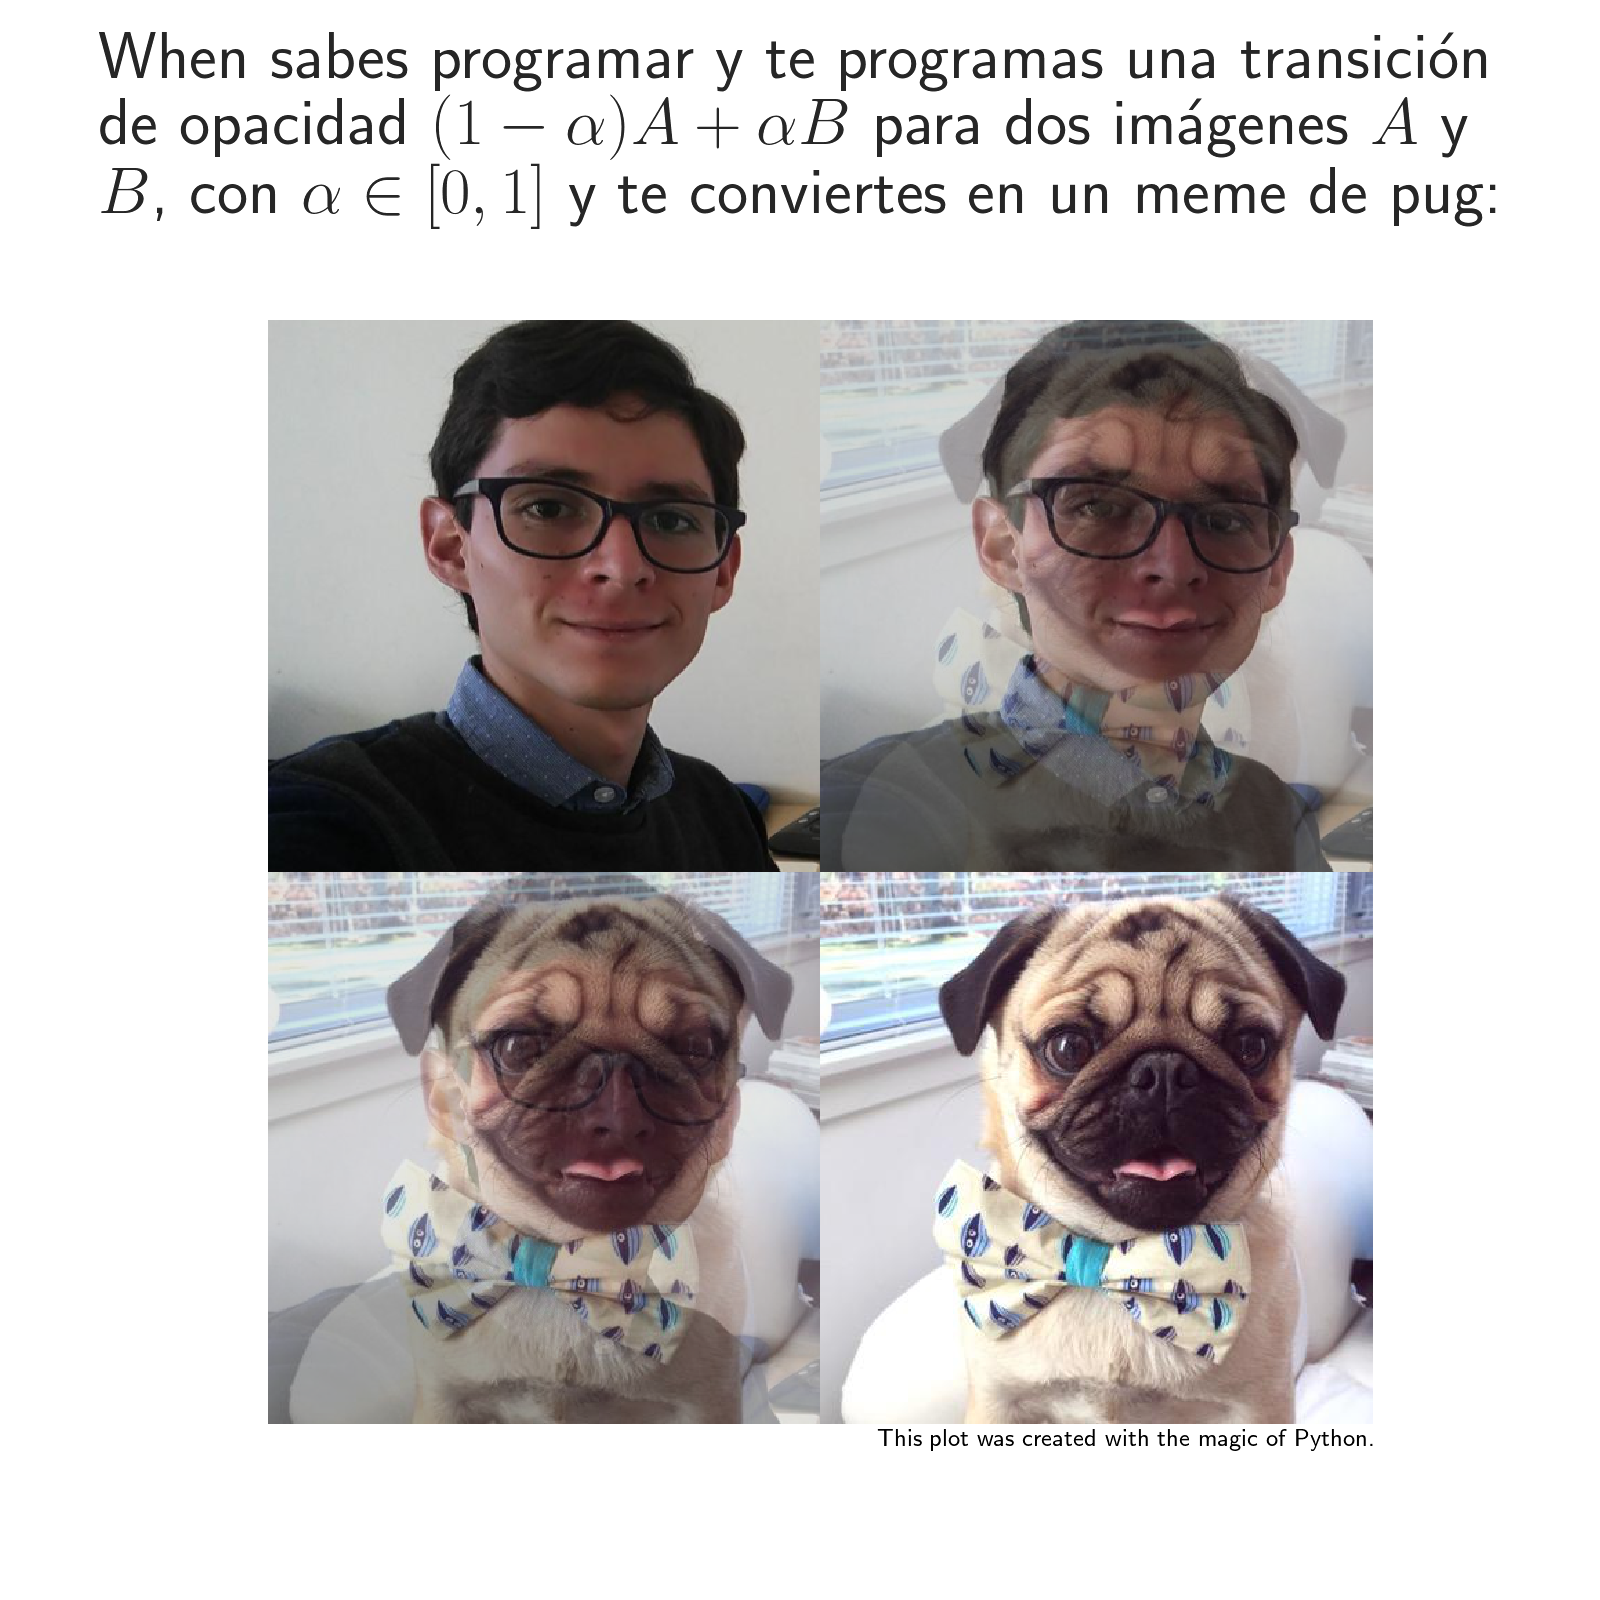
\includegraphics[width=0.48\textwidth]{imgs/meme}\hspace{0.1cm}
      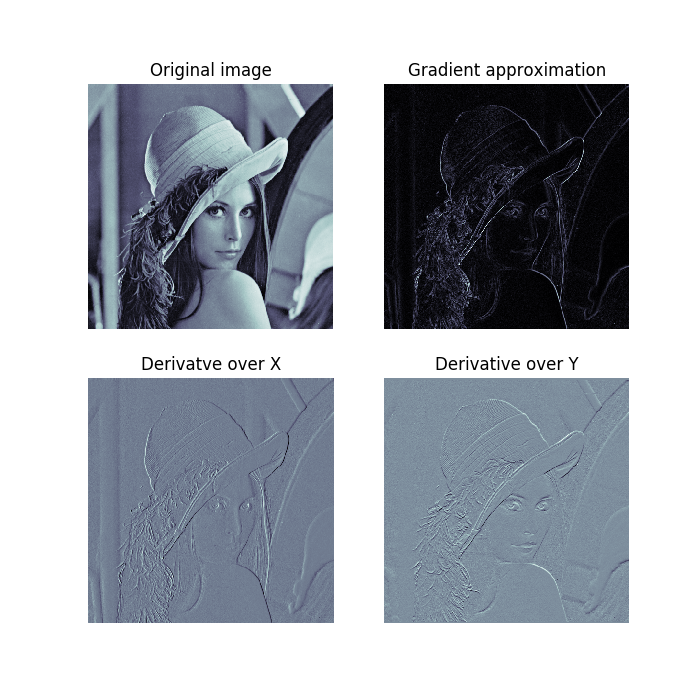
\includegraphics[width=0.48\textwidth]{imgs/derivatives}
    \end{center}
  \end{frame}

  \begin{frame}{Para ello...}
    Lo que necesitamos aprender es lo siguiente:
    \vspace*{0.5cm}
    \begin{enumerate}
      \item Desplegar una imagen
      \item Operar una imagen
      \item Realizar una transición de opacidad
      \item Acceder a pixeles y subsecciones
      \item Cortando imágenes
      \item Programar derivadas
    \end{enumerate}
  \end{frame}

  \begin{frame}{Importando \textbf{NumPy} y \textbf{Matplotlib}}
    Se pueden importar librerías simplemente haciendo \texttt{import librería},
    sin embargo, se pueden importar módulos específicos (ej. \texttt{from
    matplotlib import pyplot}) o importar módulos/librerías con un alias.\\
    \vspace*{0.3cm}
    Por simpliacidad nosotros importaremos \textbf{NumPy} y \textbf{Matplotlib}
    como sigue:
    \vspace*{0.3cm}
    \metroset{block=fill}
    \begin{block}{Importamos usando un alias:}
      \hspace{0.7cm}{\color{orange} \texttt{import }}{\color{gray} \texttt{numpy }}{\color{LimeGreen} \texttt{as }}{\color{gray} \texttt{np  }}\\
      \hspace{0.7cm}{\color{orange} \texttt{import }}{\color{gray} \texttt{matplotlib.pyplot }}{\color{LimeGreen} \texttt{as }}{\color{gray} \texttt{plt  }}\\
      \vspace*{0.5cm}
    \end{block}
  \end{frame}

  \begin{frame}{1. Desplegando una imagen}
    Matplotlib tiene una función llamada \texttt{imread}, cuyo argumento es una
    dirección y sirve para leer una imagen y guardarla como un arreglo de NumPy.\\
    \vspace*{0.3cm}
    Podemos imprimir la matriz usando la función \texttt{print} y mostrarla en
    una ventana haciendo lo que sigue:
    \vspace*{0.3cm}
    \metroset{block=fill}
    \begin{block}{Después de importar...}
      \hspace{0.7cm}{\color{gray} \texttt{img = plt.imread(}}{\color{ForestGreen} \texttt{"../imgs/Lenna.png"}}{\color{gray} \texttt{)}}\\
      \hspace{0.7cm}{\color{gray} \texttt{plt.imshow(img)}}\\
      \hspace{0.7cm}{\color{gray} \texttt{plt.show()}}\\
      \vspace*{0.5cm}
    \end{block}
    Script: \texttt{show\_img.py}
  \end{frame}

  \begin{frame}{2. Operando una imagen}
    Dado que las imágenes son matrices, es muy fácil operar imágenes utilizando
    NumPy.\\
    \vspace*{0.3cm}
    Basta hacer la operación directa en la imagen o utilizar alguna función de
    NumPy para operar:
    \vspace*{0.3cm}
    \metroset{block=fill}
    \begin{block}{Después de importar y cargar una imagen inicial...}
      \hspace{0.7cm}{\color{gray} \texttt{opr = img ** }}{\color{magenta} \texttt{0.5}}\\
      \hspace{0.7cm}{\color{gray} \texttt{opr = np.cos(img)}}\\
      \hspace{0.7cm}{\color{gray} \texttt{plt.imshow(opr)}}\\
      \hspace{0.7cm}{\color{gray} \texttt{plt.show()}}\\
      \vspace*{0.5cm}
    \end{block}
    Script: \texttt{operating\_imgs.py}
  \end{frame}

  \begin{frame}{3. Transición de opacidad}
    Una transición de opacidad para dos imágenes $A$ y $B$ está definida como
    sigue:
    $$op\_img = (1 - \alpha) \hspace*{0.2cm} A + \alpha \hspace*{0.2cm} B,$$
    tomando valores de $\alpha$ en el intervalo [0,1].\\
    \vspace*{0.3cm}
    Por ejemplo el primer estado intermedio:
    \vspace*{0.3cm}
    \metroset{block=fill}
    \begin{block}{Habiendo cargado una imagen inicial y una final...}
      \hspace{0.7cm}{\color{gray} \texttt{op\_img = }}{\color{magenta} \texttt{0.7}}{\color{gray} \texttt{*im\_i + }}{\color{magenta} \texttt{0.3}}{\color{gray} \texttt{*im\_f}}\\
      \hspace{0.7cm}{\color{gray} \texttt{plt.imshow(op\_img)}}\\
      \hspace{0.7cm}{\color{gray} \texttt{plt.show()}}\\
      \vspace*{0.5cm}
    \end{block}
    Script: \texttt{opacity.py}
  \end{frame}

  \begin{frame}{4. Accediendo a pixeles y subsecciones}
    Dado que las imágenes son matrices, accedemos a un pixel como si accediéramos
    a un elemento cualquiera de la matriz que representa a la imagen:
    $$pixel_{\{i,j\}} = img[i,j]$$

    De la misma manera, utilizando slicing podemos acceder a regiones de la
    imagen:
    $$region_{\{X\times Y\}} = img[y_i:y_j, x_i:x_j]$$
  \end{frame}

  \begin{frame}{5. Cortando una imagen}
    Con lo anterior, es muy fácil cortar y obtener una nueva imagen:
    $$region_{\{X\times Y\}} = img[y_i:y_j, x_i:x_j],$$
    simplemente hace falta guardar el resultado.\\
    \vspace*{0.3cm}
    \metroset{block=fill}
    \begin{block}{Habiendo importado librerías...}
      \hspace{0.7cm}{\color{gray} \texttt{img = plt.imread(}}{\color{ForestGreen} \texttt{"Lenna.png"}}{\color{gray} \texttt{)}}\\
      \hspace{0.7cm}{\color{gray} \texttt{cropped\_img = img[}}{\color{magenta} \texttt{220}}{\color{gray} \texttt{:}}{\color{magenta} \texttt{300}}{\color{gray} \texttt{, }}{\color{magenta} \texttt{210}}{\color{gray} \texttt{:}}{\color{magenta} \texttt{370}}{\color{gray} \texttt{]}}\\
      \hspace{0.7cm}{\color{gray} \texttt{plt.imshow(cropped\_img)}}\\
      \hspace{0.7cm}{\color{gray} \texttt{plt.show()}}\\
      \hspace{0.7cm}{\color{gray} \texttt{img = plt.imsave(}}{\color{ForestGreen} \texttt{"Lenna.png"}}{\color{gray} \texttt{, cropped\_img)}}\\
      \vspace*{0.5cm}
    \end{block}
    Script: \texttt{crop\_img.py}
  \end{frame}

  \begin{frame}{Reto para llevar}
    \vspace*{0.5cm}
    \metroset{block=fill}
    \begin{block}{Reto 1:}
      Dar formato a la transición de opacidad para que quede como sigue:\\
      \centering
      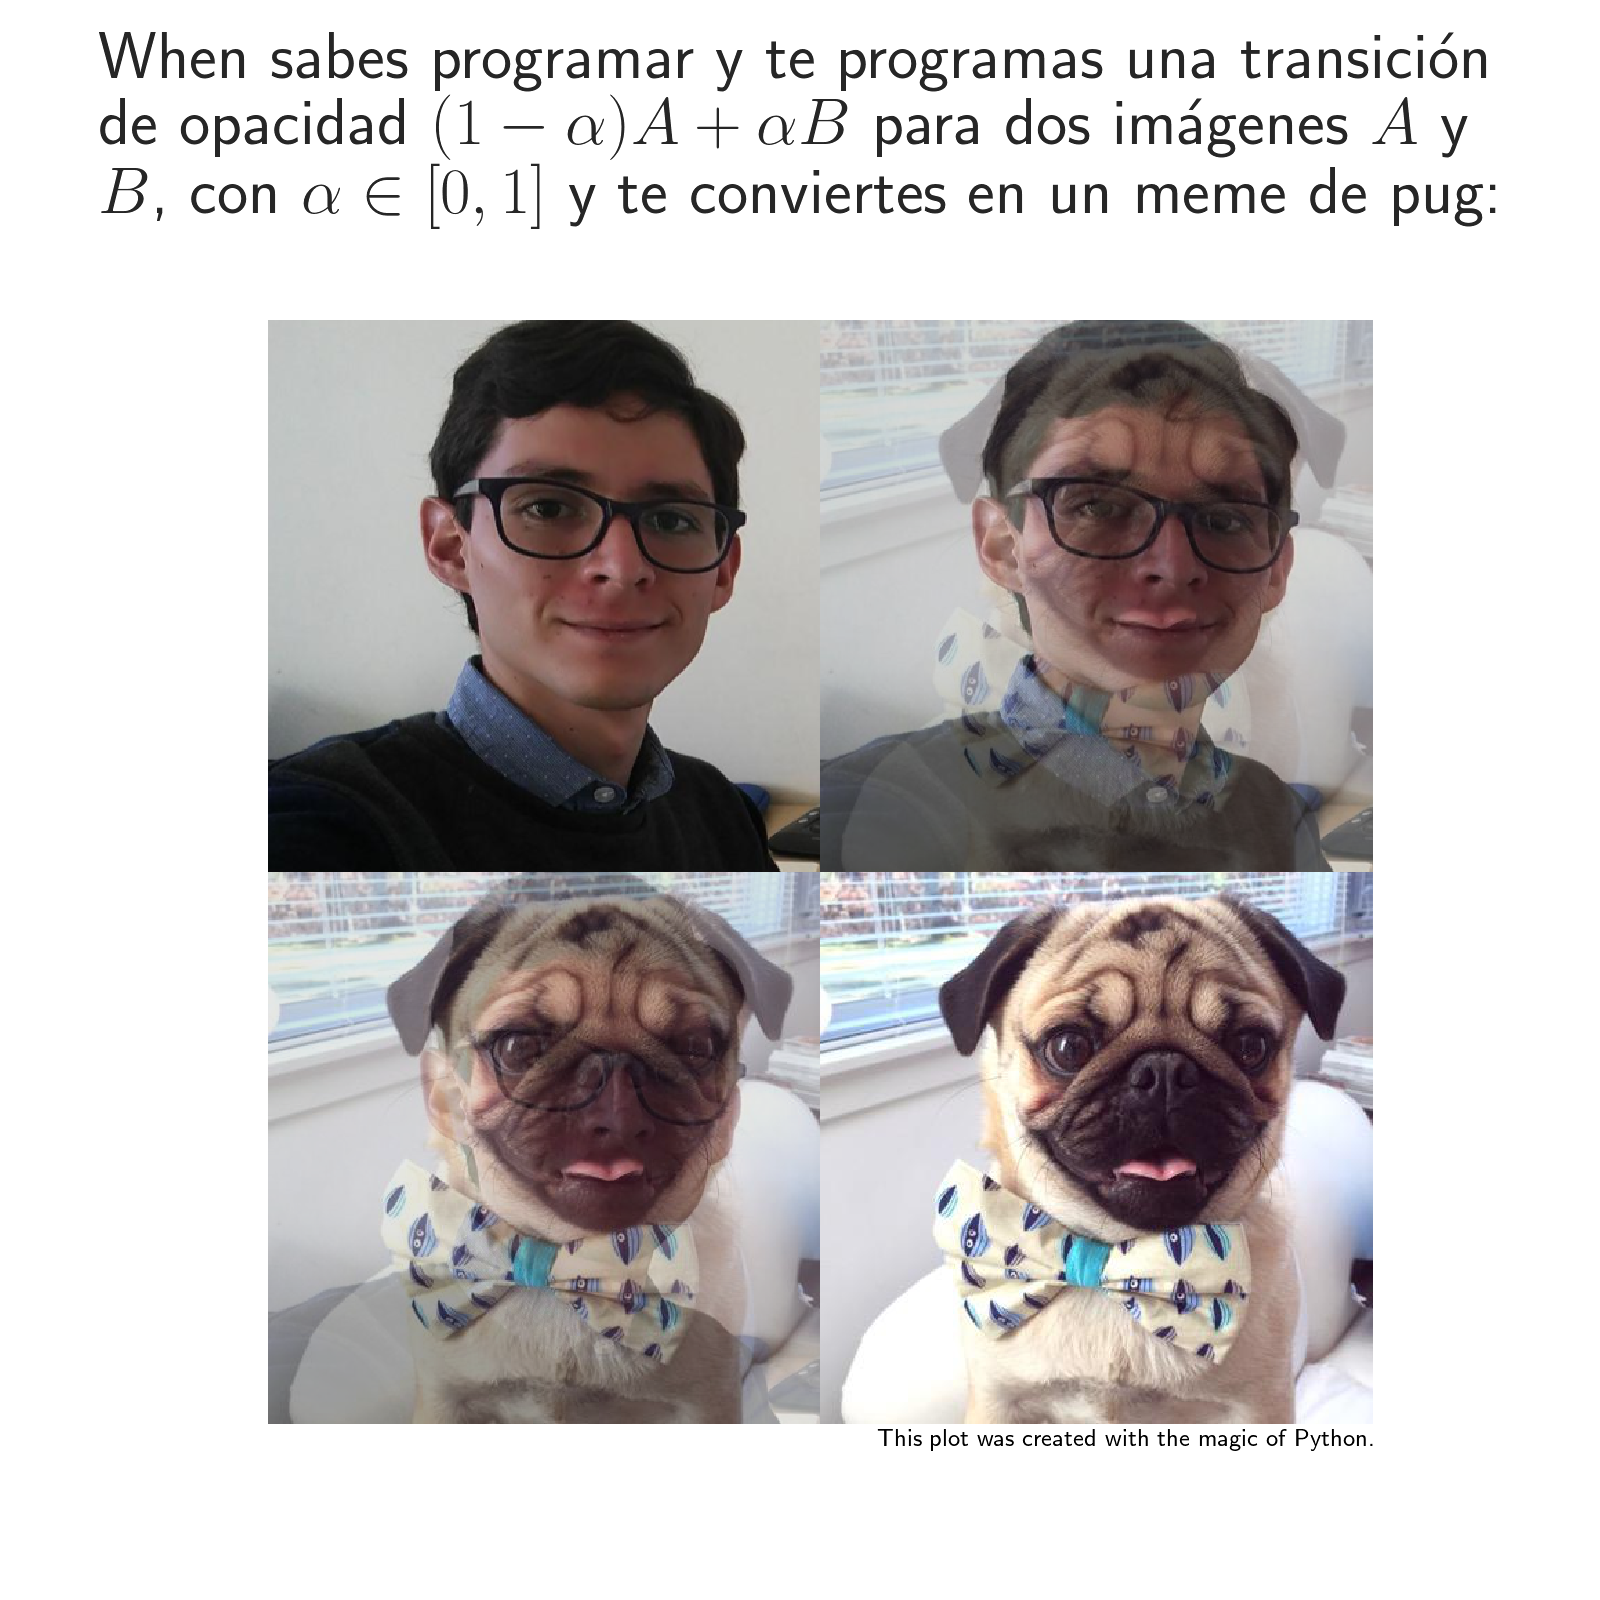
\includegraphics[width=0.48\textwidth]{imgs/meme}
      \vspace*{0.5cm}
    \end{block}
  \end{frame}

  \begin{frame}{Reto para llevar}
    \vspace*{0.5cm}
    \metroset{block=fill}
    \begin{block}{Reto 2:}
      Nuestras funciones de derivadas de imagen funcionan sólo con imágenes
      que son cuadradas, ¿por qué?\\
      \vspace*{0.5cm}
      ¿Cómo \textit{"corregir"} esto para que sirva con la imagen \texttt{leaf.png}?\\
      \centering
      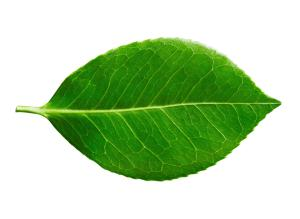
\includegraphics[width=0.48\textwidth]{../imgs/leaf}
      \vspace*{0.5cm}
    \end{block}
  \end{frame}

  \begin{frame}{Para concluir la sección...}
    Para poder concluir la sección y continuar con la siguiente,
    respondamos:
    \begin{itemize}
      \item ¿Resulta sencillo manipular imágenes (arreglos de NumPy,
      en general)?
      \item ¿Por qué las derivadas de las imágenes ayudan a
      encontrar bordes?
      \item ¿Hay alguna otra pregunta?
    \end{itemize}
  \end{frame}

  % Fifth section: Creando imágenes
  \section{Creando imágenes}
  \begin{frame}{Objetivos}
    Queremos ser capaces de recrear la siguiente imagen:
    \begin{center}
      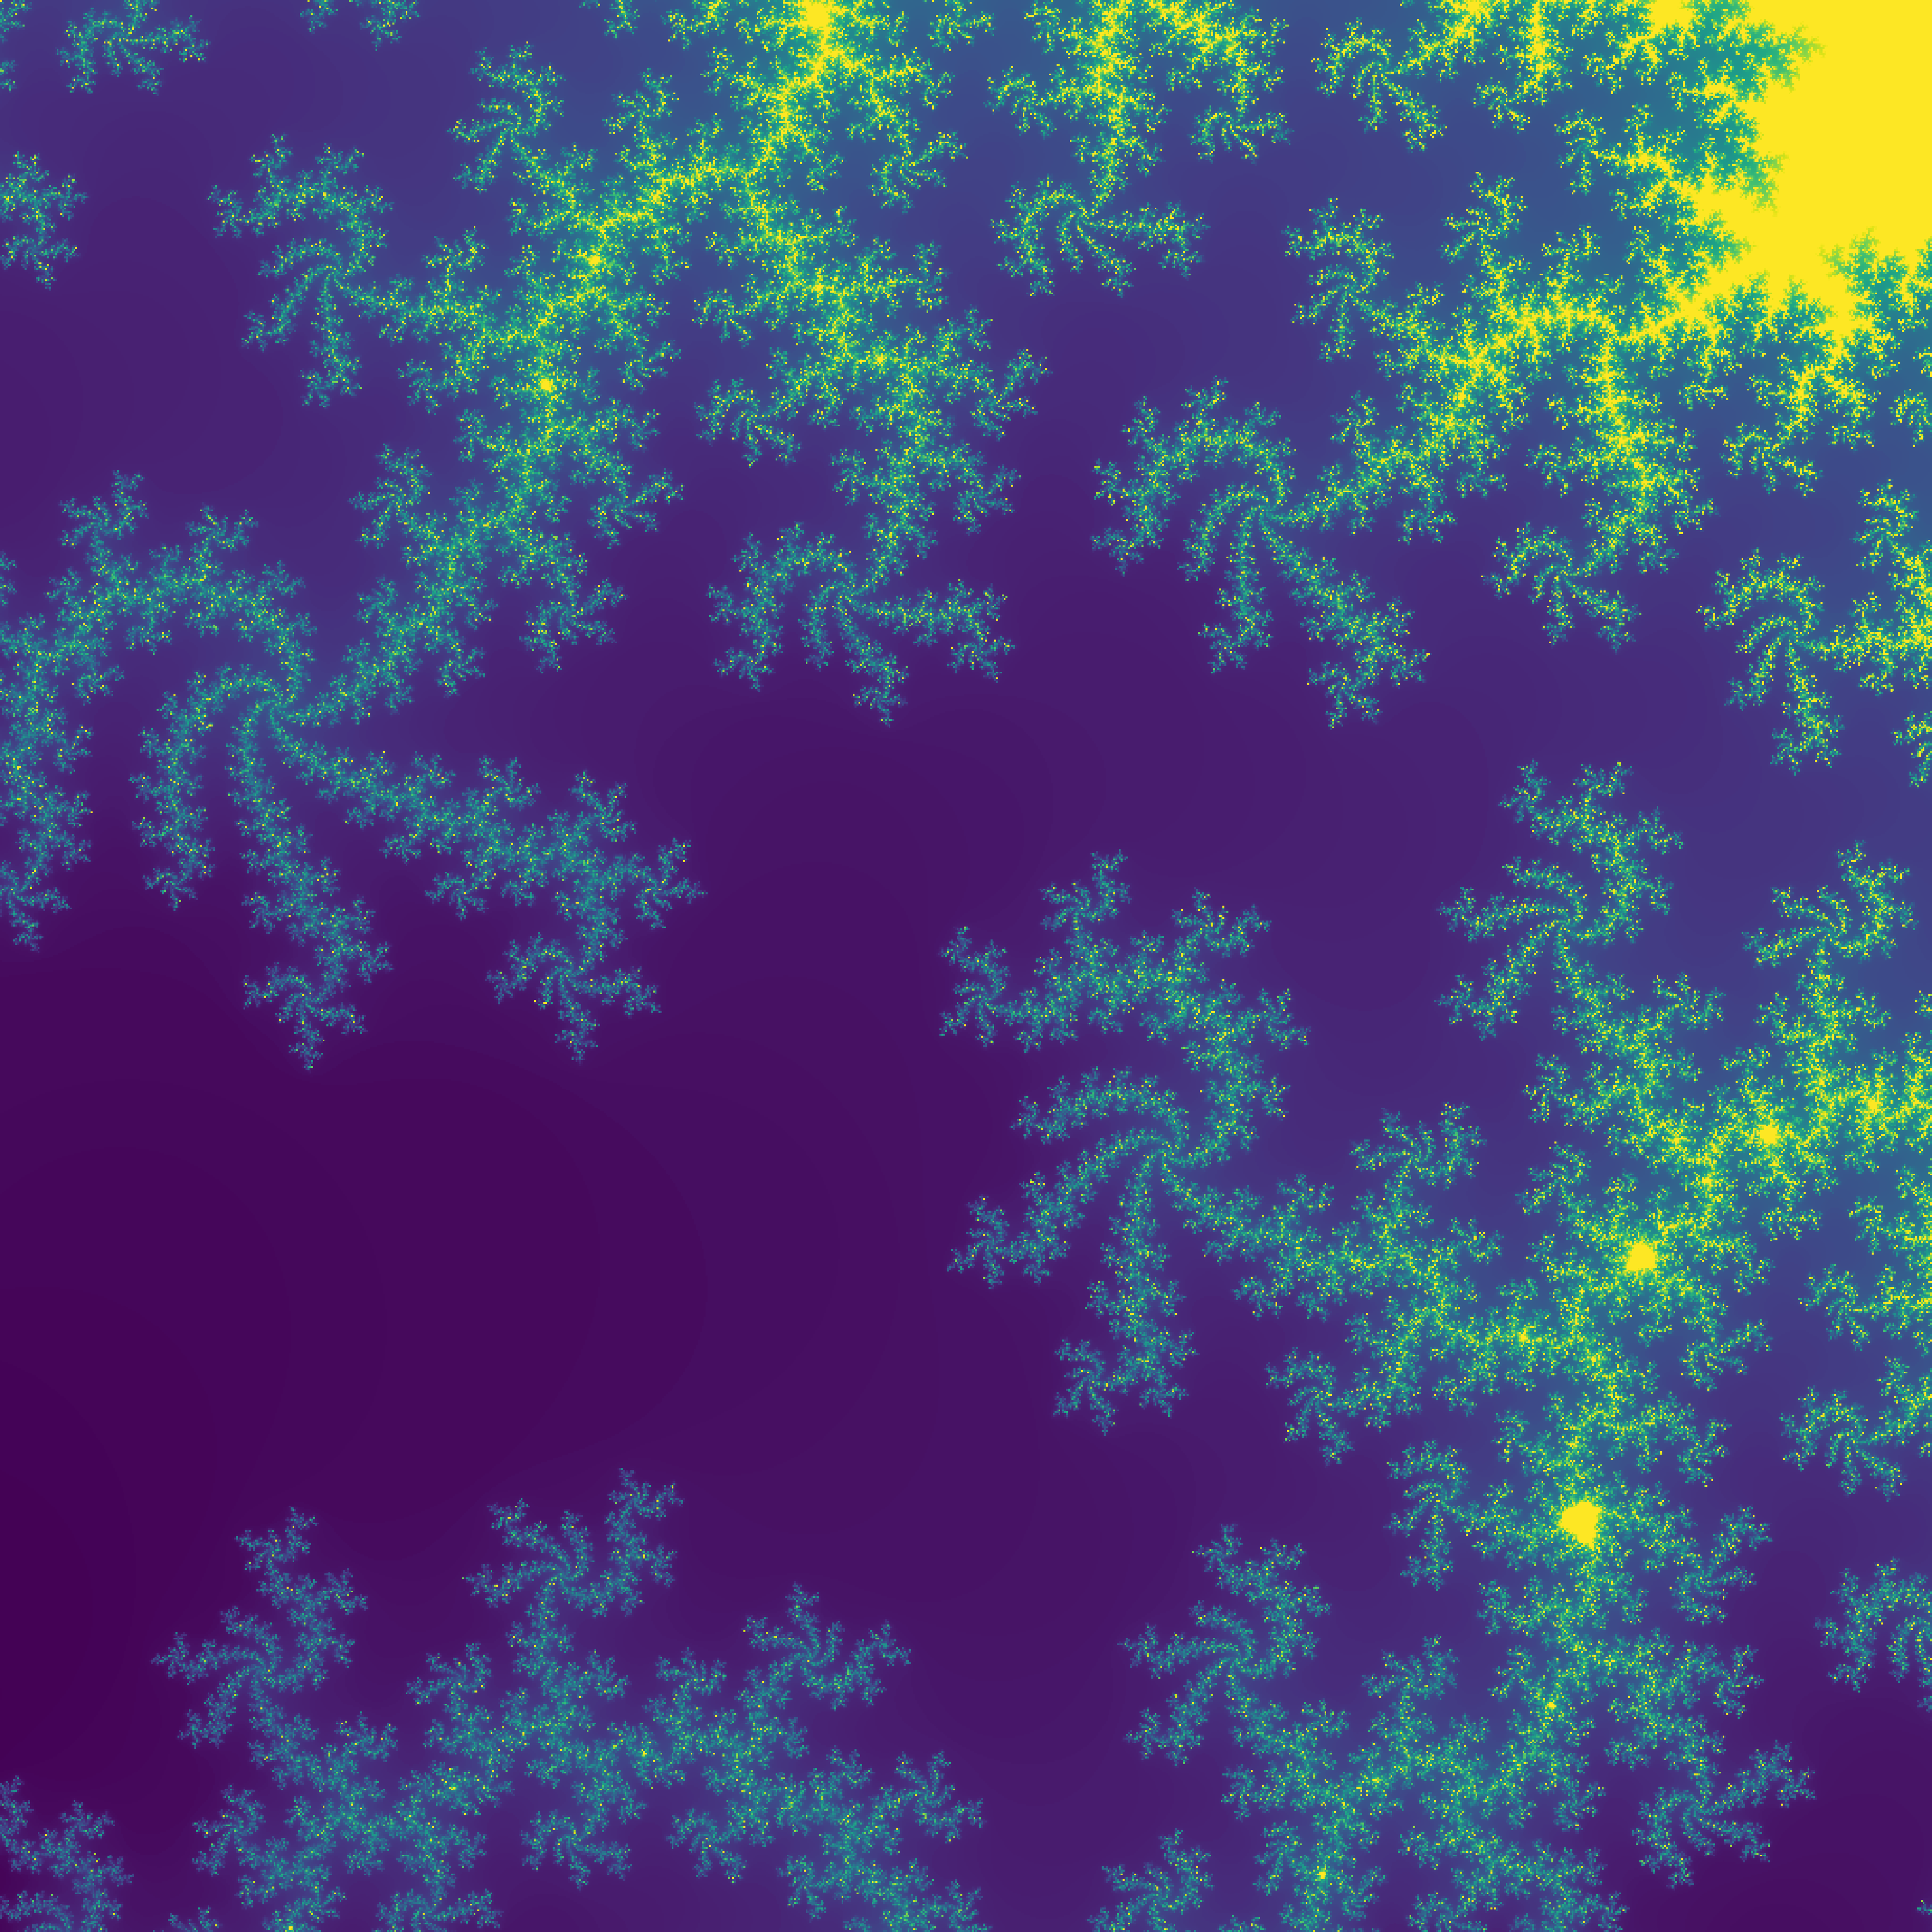
\includegraphics[width=0.6\textwidth]{imgs/mandel}\hspace{0.5cm}
    \end{center}
  \end{frame}

  % Questions
  \begin{frame}[standout]
    ¿Preguntas?
  \end{frame}

  % References
  \begin{frame}{Referencias}
    \begin{enumerate}[{[}1{]}]
      \item Python Software Foundation.\\
      \textbf{History of the software}.\\
      \textit{History and Licence},
      disponible en \texttt{https://docs.python.org/3/license.html}, 2017.

      \item Hipertextual.\\
      \textbf{¿Qué es Software Libre?}\\
      \textit{Diferencias entre Software Libre y Open Source}, 2014.

      \item Hipertextual.\\
      \textbf{¿Qué es Open Source?}\\
      \textit{Diferencias entre Software Libre y Open Source}, 2014.
    \end{enumerate}
  \end{frame}

  \begin{frame}{Referencias}
    \begin{enumerate}[{[}1{]}]
      \addtocounter{enumi}{3}

      \item The Hitchhiker's Guide to Python.\\
      \textbf{Python Imaging Library}.\\
      \textit{Image Manipulation}, 2016.

      \item The Hitchhiker's Guide to Python.\\
      \textbf{OpenSource Computer Vision}.\\
      \textit{Image Manipulation}, 2016.

      \item Python Variable Types.\\
      \textbf{Tutorials Point}.\\
      \textit{Python Basic Tutorial}.
    \end{enumerate}
  \end{frame}

  \begin{frame}{Referencias}
    \begin{enumerate}[{[}1{]}]
      \addtocounter{enumi}{6}

      \item The Hitchhiker's Guide to Python.\\
      \textbf{Python Imaging Library}.\\
      \textit{Image Manipulation}, 2016.

      \item The Hitchhiker's Guide to Python.\\
      \textbf{OpenSource Computer Vision}.\\
      \textit{Image Manipulation}, 2016.

      \item Python Variable Types.\\
      \textbf{Tutorials Point}.\\
      \textit{Python Basic Tutorial}.
    \end{enumerate}
  \end{frame}
\end{document}
